\documentclass{article}
\usepackage{graphicx} % Required for inserting images
\graphicspath{ {./IMG/} }
\usepackage{fancyhdr}
\usepackage{listings}
\usepackage{xcolor}

\definecolor{delim}{RGB}{20,105,176}
\definecolor{numb}{RGB}{106, 109, 32}
\definecolor{string_json}{rgb}{0.64,0.08,0.08}

\lstdefinelanguage{json}{
    numbers=left,
    numberstyle=\small,
    frame=single,
    rulecolor=\color{black},
    showspaces=false,
    showtabs=false,
    breaklines=true,
    postbreak=\raisebox{0ex}[0ex][0ex]{\ensuremath{\color{gray}\hookrightarrow\space}},
    breakatwhitespace=true,
    basicstyle=\ttfamily\small,
    upquote=true,
    morestring=[b]",
    stringstyle=\color{string_json},
    literate=
     *{0}{{{\color{numb}0}}}{1}
      {1}{{{\color{numb}1}}}{1}
      {2}{{{\color{numb}2}}}{1}
      {3}{{{\color{numb}3}}}{1}
      {4}{{{\color{numb}4}}}{1}
      {5}{{{\color{numb}5}}}{1}
      {6}{{{\color{numb}6}}}{1}
      {7}{{{\color{numb}7}}}{1}
      {8}{{{\color{numb}8}}}{1}
      {9}{{{\color{numb}9}}}{1}
      {\{}{{{\color{delim}{\{}}}}{1}
      {\}}{{{\color{delim}{\}}}}}{1}
      {[}{{{\color{delim}{[}}}}{1}
      {]}{{{\color{delim}{]}}}}{1},
}

\definecolor{keyword}{rgb}{0.26, 0.47, 0.85}
\definecolor{comment}{rgb}{0.5, 0.5, 0.5}
\definecolor{string_python}{rgb}{0.58, 0.0, 0.82}
\definecolor{background}{rgb}{0.95, 0.95, 0.95}

\lstdefinelanguage{Python}{
    morekeywords={def, return, import, as, if, elif, else, for, while, break, continue, pass, lambda, try, except, finally, with, yield, class, from},
    sensitive=true,
    morecomment=[l]{\#},
    morestring=[b]',
    morestring=[b]",
    morestring=[b]{'''}, % Add support for multi-line strings
    morestring=[b]{"""},
    commentstyle=\color{comment}\ttfamily,
    keywordstyle=\color{keyword}\bfseries,
    stringstyle=\color{string_python}\ttfamily,
    backgroundcolor=\color{background},
    basicstyle=\ttfamily\footnotesize,
    numbers=left,
    numberstyle=\tiny\color{gray},
    stepnumber=1,
    numbersep=10pt,
    showspaces=false,
    showstringspaces=false,
    showtabs=false,
    frame=single,
    breaklines=true,
    tabsize=4,
    captionpos=b,
    escapeinside={\%*}{*)}
}

\title{Relazione Reti StudiSync}
\author{Luca Sito 0124002612
\and Vittorio Picone 0124002584}

%\renewcommand{\headrulewidth}{0pt}
%\renewcommand{\footrulewidth}{0pt}
%\setlength\headheight{80.0pt}
%\addtolength{\textheight}{-80.0pt}



\begin{document}

\maketitle

\section{Indice}
\begin{enumerate}
    \item Traccia
    \item Introduzione
    \item Struttura
    \item Comunicazione
    \begin{enumerate}
        \item Request
        \item Give
        \item Funzioni
        \begin{enumerate}
            \item Client
            \begin{enumerate}
                \item Full Read
                \item Read Soket
                \item Client Echo
                \item Launch Method
            \end{enumerate}
        \item Server
        \begin{enumerate}
            \item Class Myhandler
            \item Class ThreadedTCPServer
            \item Server Main
        \end{enumerate}
        \end{enumerate}
       
\end{enumerate}
\item Manuale Utente
\begin{enumerate}
    \item Come Installare
    \item Login
    \item Segreteria
    \begin{enumerate}
        \item Aggiungi Corso Di Laurea
        \item Aggiungi appello
        \item Aggiungi Corso
        \item Gestisci richieste Date
        \item Gestisci prenotazioni Appelli
\end{enumerate}
\item Studente
\begin{enumerate}
    \item Richiedi Date 
    \item Richiedi Prenotazione
    \item Visualizza Storico Prenotazioni
\end{enumerate}



\end{enumerate}
\item Database
    \end{enumerate}

\section{\title{Traccia}}
Scrivere un'applicazione client/server parallelo per gestire gli esami universitari
\textbf{Segreteria}:
\begin{itemize}
    \item Inserisce gli esami sul server dell'università (salvare in un file o conservare in memoria il dato)
    \item Inoltra la richiesta di prenotazione degli studenti al server universitario
    \item Fornisce allo studente le date degli esami disponibili per l'esame scelto dallo studente
\end{itemize}
\textbf{Studente}:
\begin{itemize}
    \item Chiede alla segreteria se ci siano esami disponibili per un corso
    \item Invia una richiesta di prenotazione di un esame alla segreteria
\end{itemize}
\textbf{Server universitario}:
\begin{itemize}
    \item Riceve l'aggiunta di nuovi esami
    \item Riceve la prenotazione di un esame
\end{itemize}
Il server universitario ad ogni richiesta di prenotazione invia alla segreteria il numero di prenotazione progressivo assegnato allo studente e la segreteria a sua volta lo inoltra allo studente.

\section{\title{Introduzione}}

Il progetto è sviluppato nel linguaggio di programmazione \textbf{python} con supporto grafico mediante la libreria \textbf{pyqt5}.
Sono previsti 2 livelli di accesso: segreteria e studente; l’ autenticazione avviene tramite apposita interfaccia di login.
Il terzo attore è il server universitario che gestisce le operazioni di lettura e scrittura sul DB rispondendo in maniera parallela le richieste dai diversi Client mediante l’ utilizzo dei Socket.

\section{\title{Struttura}}

    DI seguito viene mostrata la struttura dei file nel progetto
      \begin{itemize}
          \item \textbf{Cversion}: contiene gli algoritmi in c che sono stati tradotti in python
          \item \textbf{Common}: contiene gli script comuni, come il protocollo di comunicazione
          \item \textbf{Logic}: contiene le logiche dietro le interfacce
          \begin{itemize}
              \item \textbf{Segreteria}: Contiene le logiche dietro le interfacce della segreteria
              \item \textbf{Students}: Contiene le logiche dietro le interfacce degli studenti

          \end{itemize}
          \item \textbf{db}: contiene i file CSV con i dati
          \begin{itemize}
              \item \textbf{Esami}: contiene i file che riguardano gli esami, come appelli  o corsi
              \item \textbf{Prenotazioni}: contiene i file che riguardano le richieste degli utenti
              \item \textbf{Users}; Contiene il file con le credenziali degli utenti

          \end{itemize}
          \item \textbf{deprecated}:contiene file non utilizzati nel codice
          \item \textbf{gui}: contiene i file riguardanti l' interfaccia grafica
          \begin{itemize}
              \item \textbf{Segreteria}: Contiene i file che generano le interfacce della segreteria
              \item \textbf{Students}: Contiene i file che generano le interfacce degli studenti
              \item \textbf{Designer}: contiene i file .ui generati tramite qt designer
          \end{itemize}
      \end{itemize}
\newpage
\textbf{Connessioni}

\begin{figure}
    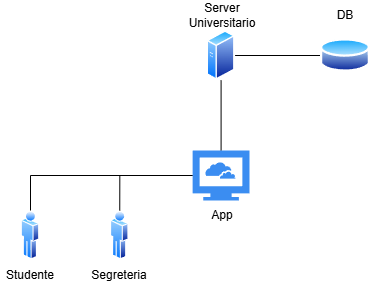
\includegraphics[width=1\linewidth]{IMG/Actors.drawio.png}
    \caption{Connessioni}
    \label{fig:wrapfig}
\end{figure}

Figure 1 Descrive come avvengono le connessioni.
I 2 diversi tipi di utenti effettuano richieste al server attraverso l' applicazione.
Il server è l' unica entità che legge e scrive sul DB

\newpage
\section{Comunicazione}
Il protocollo di comunicazione tra client e server ha come suo fondamento il formato di scambio di dati JSON. Nell'infrastrutta possiamo trovare due tipologie di JSON, \textbf{request} e \textbf{give}:
\subsection{Request}
\begin{lstlisting}[language=json,firstnumber=1]
{
  "header": "StudentsLogin",
  "payload": {
    "Matricola": "0124002584",
    "Password": "test123"
  }
}
\end{lstlisting}
Nell'esempio mostrato, si presenta un JSON \textbf{request}, formato da due attributi, \textbf{header} e \textbf{payload}, dove nell'header è presente l'endpoint richiesto, in questo caso il login per gli studenti, mentre nel payload sono presenti le informazioni necesserie al server per processare la request con successo, che in questo caso è matricola e password.
La request viene decodifica e divisa nelle sue due componenti, per poi essere passata alla funzione method\_switch, dove al suo interno è presento uno switch/case dove i case rappresentano i vari endpoint disponibili, richiamati all'interno del case con una funzione omonima all'endpoint.

\subsection{Give}
\begin{lstlisting}[language=json,firstnumber=1]
{
  "result": [
    "0124002584",
    "Vittorio",
    "Picone",
    "vittorio.picone001@studenti.uniparthenope.it",
    "1914752590",
    "0124",
    [
      "0124",
      "Informatica Triennale"
    ]
  ]
}
\end{lstlisting}
In quest altro esempio mostrato, si presenta la seconda tipologia di JSON, \textbf{give}, formato da un solo attributo, \textbf{result}, che contiene il risultato fornito dall'endpoint richiesto, che in questo caso è il risultato di un login studente andato a buon fine. I dati nell'attributo result vengono restituiti come un array, e vengono interpretati direttamente lato client. La funzione per effettuare le chiamate agli endpoint è \textbf{launchMethod}, che come parametri di input ha input (str), server\_address (str) e server\_port(int). La funzione launchMethod è stata poi abbinata per un'usabilità maggiore alle due funzioni \textbf{request\_constructor\_str} e \textbf{request\_constructor\_obj}, dove request\_constructor\_obj restituisce un JSON in formato object a request\_constructor\_str, e quest ultimo ritorna il JSON come stringa a launchMethod, avendo quindi il seguente flow operativo:
\begin{lstlisting}[language=python,firstnumber=1]
def request_constructor_obj(input_object, header):
    return {
        "header": header,
        "payload": input_object
    }


def request_constructor_str(input_object, header):
    return json.dumps(request_constructor_obj(input_object, header))

launchMethod(request_constructor_str(None, "GetCorsi"), server_coords['address'], server_coords['port']))
\end{lstlisting}

\subsection{Funzioni per la comunicazione}
\subsubsection{Client}
\begin{lstlisting}[language=python,firstnumber=1]
def full_write(fd, buf):
    nleft = len(buf)
    while nleft > 0:
        try:
            nwritten = fd.send(buf)
            nleft -= nwritten
            buf = buf[nwritten:]
        except socket.error as e:
            if e.errno == errno.EINTR:
                continue
            else:
                raise
    return nleft

async def read_socket(sock):
    received_data = ""
    while True:
        recvbuff = await asyncio.to_thread(sock.recv, MAXLINE)
        if not recvbuff:
            print("EOF on the socket")
            break
        if not recvbuff.strip():
            print("Empty data received. Closing the socket.")
            break
        received_data += recvbuff.decode()
    return received_data


async def client_echo(data, sock):
    # Write the data using full_write
    await asyncio.to_thread(full_write, sock, data.encode())
    # Wait for the socket to be flushed (optional)
    await asyncio.to_thread(sock.shutdown, socket.SHUT_WR)
    return await read_socket(sock)


def launchMethod(input: str, server_address: str, server_port: int):
    sock = socket.socket(socket.AF_INET, socket.SOCK_STREAM)

    serv_add = (server_address, server_port)

    try:
        sock.connect(serv_add)
        print(f"Connection to {serv_add} established!")
    except Exception as e:
        print(f"Connection error: {e}")
        sys.exit(1)

    result = asyncio.run(client_echo(input, sock))

    # Close the socket after finishing the data stream
    sock.close()

    return result
\end{lstlisting}
\paragraph{full\_write(fd, buf)}
Questa funzione ha il compito di inviare tutti i dati presenti nel buffer buf sul file descriptor fd (in questo caso, una socket). Ecco come funziona:

\begin{enumerate}
\item Calcolo di nleft: Viene calcolata la lunghezza dei dati da inviare.
\item Ciclo while: Continua finché ci sono dati da inviare (nleft > 0).
\item Tentativo di invio dati: Utilizza fd.send(buf) per inviare i dati.
\item Aggiornamento variabili: Sottrae il numero di byte inviati (nwritten) da nleft e aggiorna buf per rimuovere i dati già inviati.
\item Gestione errori: Se si verifica un'eccezione di tipo socket.error, controlla se l'errore è errno.EINTR (interruzione del sistema). In tal caso, il ciclo continua; altrimenti, l'eccezione viene rilanciata.
\end{enumerate}



\paragraph{read\_socket(sock)}
Questa funzione asincrona legge i dati da una socket finché non riceve EOF (End Of File) o dati vuoti:

\begin{enumerate}
\item Inizializzazione di received\_data: Una stringa vuota per accumulare i dati ricevuti.
\item Ciclo while: Continua indefinitamente.
\item Lettura dati: Usa asyncio.to\_thread per eseguire sock.recv in un thread separato e attendere il risultato.
\item Controllo EOF: Se non vengono ricevuti dati (not recvbuff), stampa un messaggio e interrompe il ciclo.
\item Controllo dati vuoti: Se i dati ricevuti sono vuoti, stampa un messaggio e interrompe il ciclo.
\item Accumulo dati: Aggiunge i dati decodificati a received\_data.
\item Ritorno dei dati ricevuti: Al termine del ciclo, restituisce received\_data.
\end{enumerate}

\paragraph{client\_echo(data, sock)}
Questa funzione asincrona invia dei dati ad un server e legge la risposta:

\begin{enumerate}
\item Invio dati: Utilizza asyncio.to\_thread per eseguire full\_write in un thread separato, inviando i dati codificati (data.encode()) tramite la socket.
\item Chiusura socket: Chiude il canale di invio della socket (sock.shutdown(socket.SHUT\_WR)).
\item Lettura risposta: Attende e ritorna la risposta dal server tramite read\_socket(sock).
\end{enumerate}

\paragraph{launchMethod(input: str, server\_address: str, server\_port: int)}
Questa funzione avvia la comunicazione con il server:

\begin{enumerate}
    \item Creazione della socket: Crea una socket TCP/IP.
    \item Costruzione dell'indirizzo del server: Crea una tupla con l'indirizzo e la porta del server.
    \item Connessione al server: Tenta di connettersi al server e stampa un messaggio di conferma.
    \item Gestione errori di connessione: In caso di errore durante la connessione, stampa un messaggio e termina il programma.
    \item Usa asyncio.run per eseguire la funzione client\_echo e attende il risultato.
    \item Chiude la socket.
    \item Restituisce il risultato ottenuto da client\_echo.
\end{enumerate}

\subsubsection{Server}
\begin{lstlisting}[language=python,firstnumber=1]
class MyHandler(socketserver.StreamRequestHandler):
    def handle(self):

        host, port = self.client_address
        print(f"Request from host {host}, port {port}")

        while True:
            try:
                data = self.rfile.readline(MAXLINE)
                if not data:
                    print(f"Connection closed by {self.client_address}")
                    break

                print(f"Received from {self.client_address}: {data}")
                data_decoded = data.decode().replace('\n', '')
                data_decoded = json.loads(data_decoded)

                print(f"Parsed Data: {data_decoded}")

                result = method_switch(data_decoded["header"], data_decoded["payload"])
                response = f"{json.dumps(result)}".encode("utf-8")
                print(f"Response to send: {response}")

                # Use blocking send to ensure the response is fully sent before closing
                sent = full_write(self.request, response)
                print(f"Sent {sent}")

            except socket.error as e:
                if e.errno == 10054:
                    print(f"Connection forcibly closed by the remote host {self.client_address}")
                else:
                    print(f"{bcolors.FAIL} Socket Error: {e}{bcolors.ENDC}")
                break
            except Exception as e:
                print(f"{bcolors.FAIL} Generic Exception Error: {e}{bcolors.ENDC}")
                break


class ThreadedTCPServer(socketserver.ThreadingMixIn, socketserver.TCPServer):
    pass


def server_main(server_address, server_port):
    server = ThreadedTCPServer((server_address, server_port), MyHandler)
    server_thread = threading.Thread(target=server.serve_forever)
    server_thread.start()
    print(f"Server listening on port {server_port}...")

    try:
        server_thread.join()
    except KeyboardInterrupt:
        print("Server terminated by user")
\end{lstlisting}

\paragraph{Class MyHandler}
\begin{enumerate}
    \item Identificazione del client: Stampa l'indirizzo del client connesso.
    \item Ciclo di lettura dei dati: Continua a leggere dati dal socket finché non viene chiusa la connessione.
    \begin{enumerate}
        \item Lettura dei dati: Legge una linea di dati dalla socket.
        \item Chiusura della connessione: Se non ci sono dati, la connessione è chiusa.
        \item Decodifica e parsing dei dati: I dati ricevuti sono decodificati da bytes a stringa e poi convertiti in un oggetto JSON.
        \item Elaborazione della richiesta: Usa method\_switch per elaborare i dati e ottenere un risultato.
        \item Invio della risposta: Codifica il risultato in bytes e lo invia al client usando full\_write.
        \item Gestione degli errori: Gestisce eventuali errori di socket e generici, stampando messaggi di errore colorati.
    \end{enumerate}
\end{enumerate}

\paragraph{Classe ThreadedTCPServer}
Questa classe estende TCPServer e ThreadingMixIn per permettere la gestione multithreading delle richieste

\paragraph{Funzione server\_main}

\begin{enumerate}
    \item Creazione del server: Crea un'istanza di ThreadedTCPServer con l'indirizzo e la porta specificati.
    \item Avvio del thread del server: Avvia un thread separato per eseguire il server in modo che possa gestire le richieste in arrivo.
    \item Messaggio di ascolto: Stampa un messaggio indicando che il server è in ascolto sulla porta specificata.
    \item Attesa del thread: Usa join per mantenere il programma in esecuzione finché il thread del server è attivo.
    \item Gestione dell'interruzione: Gestisce l'interruzione da tastiera (KeyboardInterrupt) per permettere all'utente di terminare il server pulitamente.
\end{enumerate}

\newpage

\section{Manuale Utente}
\subsection{Come Installare}
Linux Distrubution: Ubuntu
\begin{enumerate}
    \item Aggiorna sudo: sudo update poi sudo upgrade
    \item Aggiorna le librerie: sudo apt install build-essential zlib1g-dev libncurses5-dev libgdbm-dev libnss3-dev libssl-dev libreadline-dev libffi-dev libsqlite3-dev wget libbz2-dev
    \item Scarica python 3.11: wget https://www.python.org/ftp/python/3.11.0/Python-3.11.0.tgz
    \item Estrai il file scaricato: tar -xf Python-3.11.0.tgz
    \item Vai nella cartella: cd Python-3.11.0
    \item Ottimizza la build ./configure --enable-optimizations
    \item Assegnamo più processori per velocizzare la build: make -j\$(4)
    \item installa: sudo make altinstall
    \item per sicurezza vediamo se lì installazione è avvenuta con successo: python3.11 --version
    \item installiamo git: se sei su ubuntu: sudo apt install git-all altrimenti: sudo dnf install git-all
    \item clona il progetto:  git clone https://github.com/VikSn0w/StudiSync.git (verranno richieste le credenziali o un access token)
    \item Spostati nell directory del progetto: cd <dirProgetto>
    \item Creiamo un venv: python3 -m venv .venv
    \item Entiamo nel venv: source .venv/bin/activate
    \item Installa le librerie: pip install -r requirements.txt
    \item Installiamo dipendenze: 
    sudo apt-get install libxcb-xinerama0
    
    sudo apt-get install libxkbcommon-x11-0 libxcb-icccm4 libxcb-image0 libxcb-keysyms1 libxcb-randr0 libxcb-render-util0 libxcb-xinerama0 libxcb-xfixes0 libegl1-mesa
    \item Avvia il server: python combined\_multiplex\_concurrent\_server.py
    \item Avvia il main: python main.py
\end{enumerate}

\newpage

\subsection{Login}

Figura 2 rappresenta l' intrfaccia di login, si necessita di inserire email/matricola in caso
di studente e password personale, gli utenti vengono inseriti manualmente nei file CSV con le password crittogarfate tramite un algoritmo custom. Bisogna inoltre specificare la tipologia di utente che sta eseguendo l' accesso


\begin{figure}
    \centering
    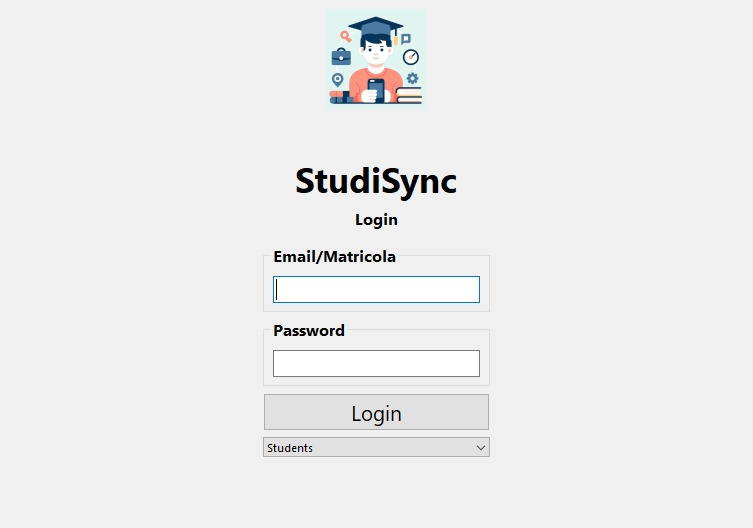
\includegraphics[width=1\linewidth]{IMG/loging_interface.jpg}
    \caption{Interfaccia Login}
    \label{fig:enter-label}
\end{figure}


Se le credenziali inserite sono corrette si apre l' interfaccia Home dell' utente selezionato, altrimenti si ottiene un messaggio di errore "email, password or user type incorrest. Check your info and retry"

\subsection{Segreteria}

\begin{figure}
    \centering
    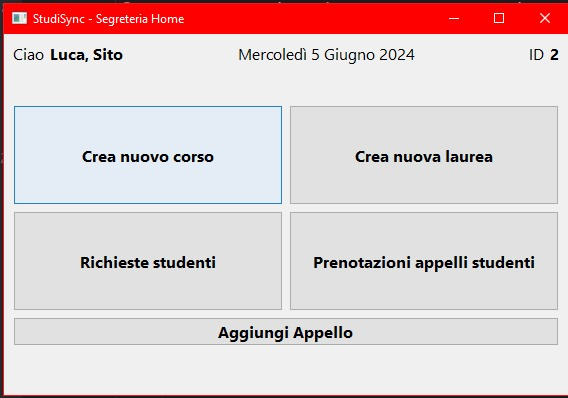
\includegraphics[width=0.75\linewidth]{IMG/HomeSegreteria.jpg}
    \caption{Home segreteria}
    \label{fig:enter-label}
\end{figure}

Quando un utente della segreteria effettua il login, viene mostrata questa interfaccia dove è possibile accedere a tutte le funzionalità

\newpage

\subsubsection{Aggiungi Corso Di Laurea}
\newpage
\begin{figure}
    \centering
    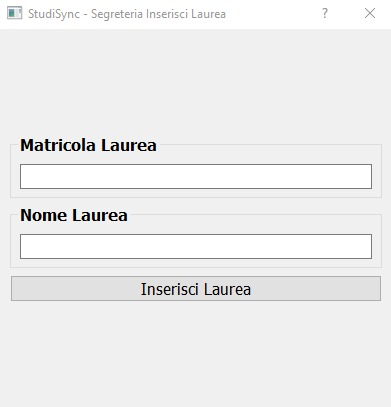
\includegraphics[width=\linewidth]{IMG/inserisciLurea.jpg}
    \caption{Aggiungi Laurea}
    \label{fig:enter-label}
\end{figure}
La figura 4 mostra l' interfaccia aggiungi corso di laurea, i campi richiesti sono la matricola e il nome di riconoscimento della laurea. Una volta inserititi  i dati e premuto sul pulsante "Inserisci laurea", verrà mostrato un messaggio di avvenuto inserimento del corso di laurea se non si verifica nessun errore.

\subsubsection{Aggiungi Appello}
\begin{figure}
    \centering
    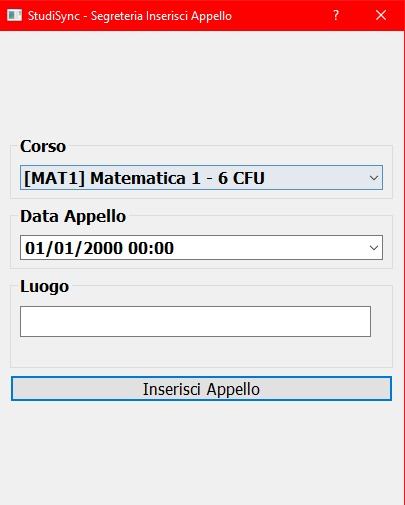
\includegraphics[width=0.75\linewidth]{IMG/InserisciAppello.jpg}
    \caption{Inserisci Appello}
    \label{fig:enter-label}
\end{figure}

\newpage
La figura 5 mostra l' interfaccia inserisci appello, i campi richiesti sono
\begin{itemize}
    \item Il corso del quale si vuole aggiungere un appello, selezionabile tramite menù a tendina, verranno mostrati i corsi aggiunti in precedenza tramite le funzione "Aggiungi Corso"
    \item Data e ora dell' appello 
    \item Luogo in cui si effettuerà la prova
\end{itemize}

Una volta inserititi  i dati e premuto sul pulsante "Inserisci appello", verrà mostrato un messaggio di avvenuto inserimento dell'appello se non si verifica nessun errore.

\newpage
\subsubsection{Aggiungi Corso}
\begin{figure}
    \centering
    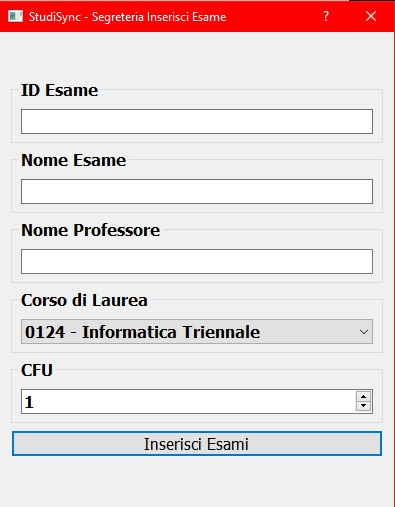
\includegraphics[width=0.75\linewidth]{IMG/aggiungiEsame.jpg}
    \caption{Aggiuingi Corso}
    \label{fig:enter-label}
\end{figure}

La figura 6 mostra l' interfaccia aggiungi Corso, i campi richiesti sono:
\begin{itemize}
    \item Id esame, un codice univoco che identifica l' esame
    \item Nome esame, il nome del' esame
    \item Nome proefessore che tiene in corso
    \item  Corso di leurea, selezionabile tramite il menù a tendina, si possono scegliere i corsi precedentemente inseriti 
    \item Numero di CFU riconosciuti per quell' esame
\end{itemize}

\begin{figure}
    \centering
    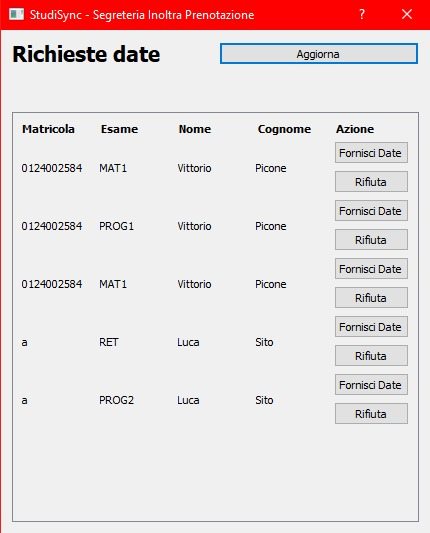
\includegraphics[width=1\linewidth]{IMG/richiesteDate.jpg}
    \caption{Richiesrte date}
    \label{fig:enter-label}
\end{figure}
\subsubsection{Gestisci Richieste Date}
la figura 7 mostra l' interfaccia "richieste date" Qui sono riportate tutte le richieste di date effettuate dagli studenti, per ogni richiesta è possibile:
\begin{itemize}
    \item Fornire le date: Il server si occuperà di fornire le date dell' esame richiesto allo studente, che potrà visualizzarle dalla sua interfaccia
    \item Rifiutare: lo studente non otterrà le date e potrà visualizzare la sua proposta come "Rifiutata"
\end{itemize}

A prescindere dalla scelta, la riga con la richiesta verrà eliminata dalla tabella e verrà mostrato un messaggio in base all' esito dell' elaborazione
\newpage

\begin{figure}
    \centering
    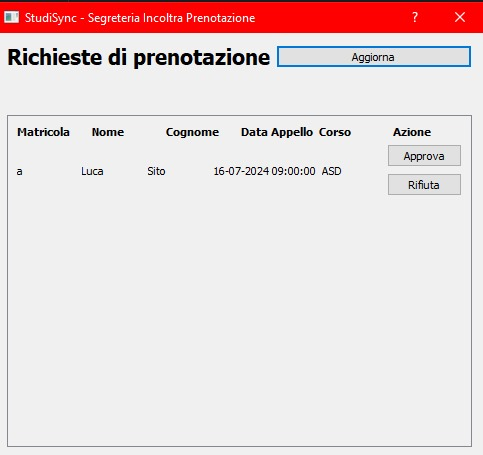
\includegraphics[width=1\linewidth]{IMG/RIchiestePrenotazioni.jpg}
    \caption{Richieste Prenotazioni}
    \label{fig:enter-label}
\end{figure}
\subsubsection{Gestisci Prenotazioni Appelli}
la figura 8 mostra l' interfaccia "richieste prenotazione" Qui sono riportate tutte le richieste di  prenotazione effettuate dagli studenti, per ogni richiesta è possibile:
\begin{itemize}
    \item Approvare: Lo studente visualizzera lo stato della sua richiesta come "evasa" e quindi è a tutti gli effetti prenotato all' esame
    \item Rifiutare: Lo studente vedrà dalla sue interfaccia "Respinta" e drovrà effettuare un altra richiesta per essere accettato.
\end{itemize}

A prescindere dalla scelta, la riga con la richiesta verrà eliminata dalla tabella e verrà mostrato un messaggio in base all' esito dell' elaborazione

\subsection{Studente}
\begin{figure}
    \centering
    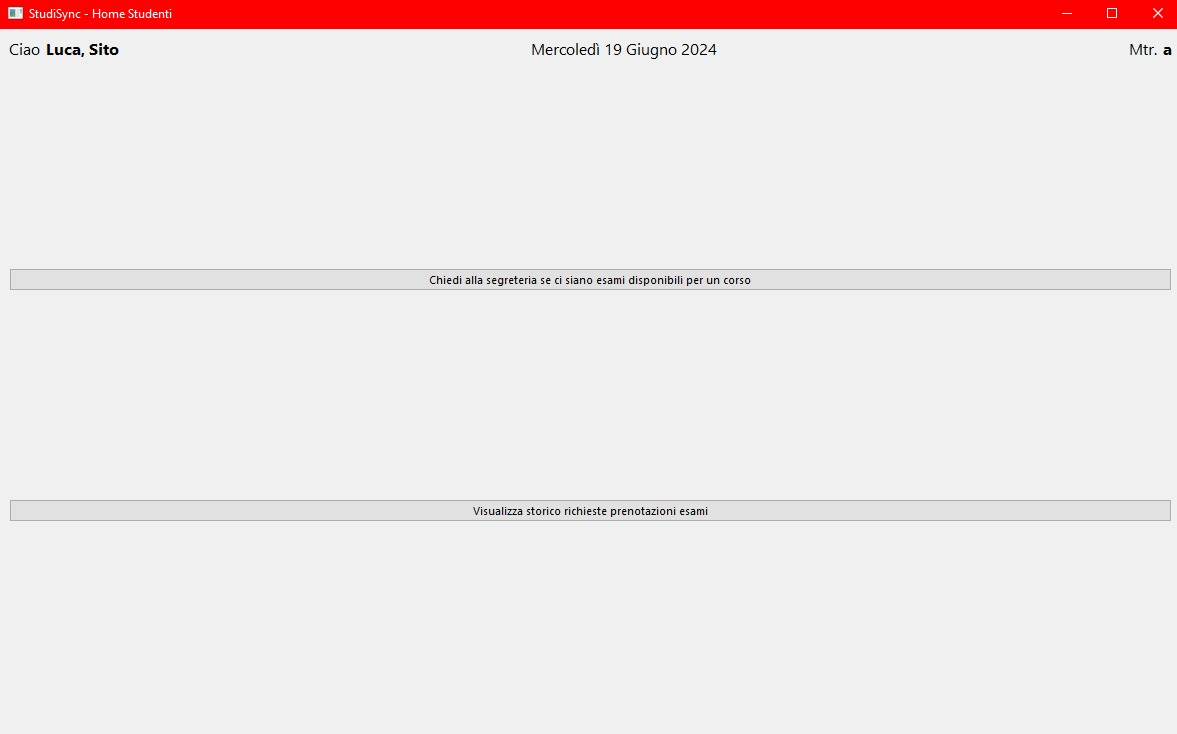
\includegraphics[width=1\linewidth]{IMG/studentehome.jpg}
    \caption{Enter Caption}
    \label{fig:enter-label}
\end{figure}
Quando un utente studente effettua il login, viene mostrata questa interfaccia dove è possibile accedere a tutte le funzionalità
\newpage

\subsubsection{Richiedi date}
\begin{figure}
    \centering
    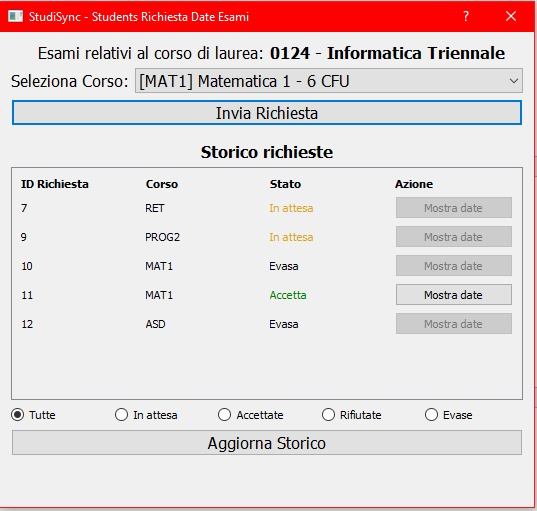
\includegraphics[width=1\linewidth]{IMG/richiediDate.jpg}
    \caption{Richiedi date}
    \label{fig:enter-label}
\end{figure}
La figura 10 mostra l' interfaccia "richiedi date", dove è possibile fare richiesta alla segreteria per sapere le date disponibili per un dterminato esame, per fare richiesta basta:
\begin{enumerate}
    \item selezionare l' esame interessato tramite il menù a tendina 
    \item Fare click su invia richiesta
\end{enumerate}

E' possibile inoltre visualizzare uno storico di tutte le richieste inviate in precedenza. 
Le richieste possono avere i seguenti stati:
\begin{itemize}
    \item In attesa: la segreteria ha ricevuto la richiesta ma ancora deve approvarla/respingerka
    \item Accettata: la segreteria ha accettato la richiesta e sono state fornite le date di appello per quell' esame
    \item Rifiutata: la segreteria ha respinto la richiesta
    \item Evasa: la segreteria ha accettato non solo la richiesta di date ma anche la prenotazione ad un appello in una determinata data

\end{itemize}

E' possibile filetrare le richieste per status

\newpage

\begin{figure}
    \centering
    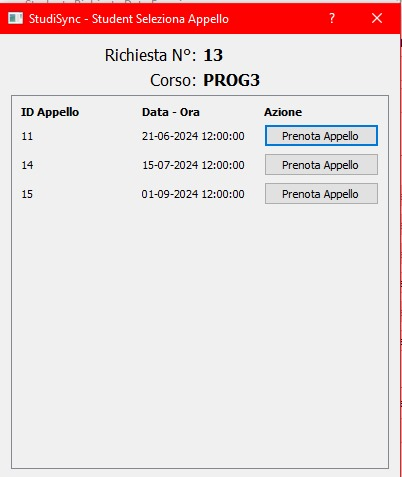
\includegraphics[width=0.8\linewidth]{IMG/RichiediPrenotazioneAppello.jpg}
    \caption{Richiedi Prenotazione}
    \label{fig:enter-label}
\end{figure}

\subsubsection{Richiedi prenotazione}

In figura 11 viene mostrata l' interfaccia "Richiedi prenotazione", questa interfaccia può essere raggiunta cliccando su "mostra date" in figura 10, dopo che la segreteria ha fornoto le date richieste per un determinato esame.
Per prenotarsu all' appello basta cliccare su "Prenota appello" sulla riga che si desidera in base alla data dell' appello.
In seguito la segreteria dovrà accettare/riufiutare la richiesta di prenotazione


\newpage
\begin{figure}
    \centering
    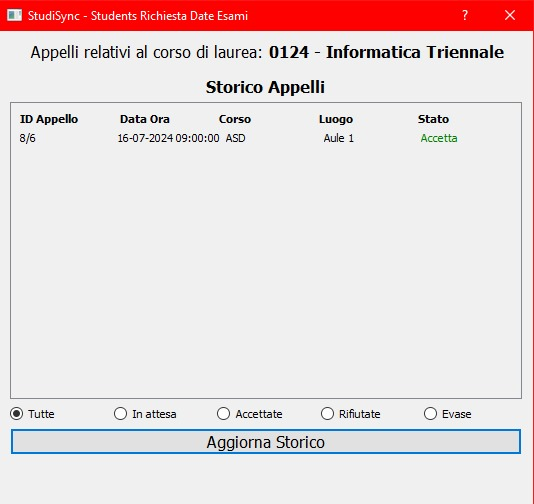
\includegraphics[width=1\linewidth]{IMG/storico_prenotazioni.jpg}
    \caption{Storico Prenotazini}
    \label{fig:enter-label}
\end{figure}

\subsubsection{Visualuzza Storico Prenotazioni}
In figura 12 viene mostata l' interfaccia "Storico Prenotazioni" dove è possibile vedere lo storico delle prenotazioni passate con tanto di stato, è anche possibile filtrare per stato


\section{Database}
Il sistema utilizzato non rispecchia completamente la definizione di database, ma comunque vengono predisposte delle procedure per un' accesso rapido ai dati organizzati su dei file CSV, ai quali solamente il server più accedervi sia in lettura che in scrittura.

Visto l' ambiente di programmazione concorrente l' accesso ai file avviene in una sezione critica tra i processi figli del server, solo le operazioni di scrittura avvengono in sezione critica.

La mutua esclusione è stata imlementata tramite la classe Lock() presente nella libreria nativa di python 3.11 "multiprocessing";
per ottenere la mutua esclusione:
\begin{enumerate}
    \item Si instanzia la classe Lock:  locker = multiprocessing.Lock
    \item Si utilizza acquire all' inizio della sezione crititca: locker..aquire()
    \item Si scrive il codice nella sezione critica
    \item Si rilascia: locker.relese()

\end{enumerate}

Ergo Lock() funge da mutex garantendo anche la mutua escusione


\end{document}
